\subsection{IllustrisTNG}
IllustrisTNG \footnote{https://www.tng-project.org/} is the follow-up project after the success of the Illustris simulations \parencite{Springel2017, Pillepich2017,Naiman2018, Nelson2017, Marinacci2018}. It is a huge project, built upon a magneto-hydrodynamical cosmological simulation code with added physical processes on a subgrid level \parencite{Weinberger2016}. Adding physical processes like gas radiation, star formation, stellar feedback through supernova explosions, supermassive black hole accretion and magnetic fields is essential to model galaxy formation and evolution and allows for a much better comparison to reality than dark matter-only simulations. The data output from the simulations is extensive, and is not meant to be analyzed all in one go, but rather through a series of analyzes, each targeting a specific scientific question. 

Hydrodynamical cosmological simulations are used to predict the movements and interactions between different types of particles in a cosmological box, and follow these through time steps as the simulation progresses. In the end, the simulation gives information about the final particle positions and properties. The simulation does not know about halos, so the raw data must be processed to extract information about separate halos and galaxies. To identify which particles belong together as one halo, their closeness has to be examined, as well as their velocities to see if their kinetic energy is enough to make them gravitationally unbound. Several different halo-finding alogrithms have been developed for this purpose, and in TNG the SUBFIND algorithm has been used.

SUBFIND is an algorithm presented in \textcite{Springel2001} for identifying halos and subhalos. It first defines parent halos with a Friends-Of-Friends algorithm, which determines halos by the proximity of the particles only. It then looks at the halo's density fields and separates out subhalos. Finally physically unbound particles (those with positive total energy) are removed. Subhalos identified to reside inside a larger subhalo are counted as a seperate subhalo, and thus its particles are not part of the parent subhalo. The relative mass of a parent subhalo compared to that of any subhalos contained within it is usually such that the impact of removing the latter is minimal with respect to any properties of the former.


\subsubsection{The simulations}
The IllustrisTNG project includes 18 different simulations with varying resolutions, spatial size, and included physics. There are three main simulations, TNG300, TNG100, and TNG50, that differ in volume and resolution. The details of these are summed up in Table \ref{TNG}. Each of the main simulations has been run at three different resolution levels, which makes it possible to study how the outcome is affected by changing only the resolution in a given simulation. TNG100 has a physical box volume of $110.7^3 \, $Mpc$^3$, and a baryonic particle resolution of $1.4 \times 10^6 M_{\odot}$, while the TNG300 simulation has a volume of $302.6^3 \, $Mpc$^3$ and a baryonic particle resolution of $1.1 \times 10^7 M_{\odot}$. The newly released third simulation, TNG50, has a smaller volume of $51.7^3 \, $Mpc$^3$, but with a much higher baryonic particle resolution of $8.5 \times 10^4 M_{\odot}$. 

In this project, a large statistical sample of galaxies was needed, as well as resolved structure of the inner part of the galaxies to calculate the different properties, so the TNG100 simulation was the best choice with respect to size and resolution. The TNG100-1 simulation data, which is the highest available resolution for TNG100, has been used throughout the project and will from now on be referred to as TNG only. A visual representation of parts of the simulations can be seen in Figure \ref{tng_illustration}. For its cosmology parameters TNG uses the results from the Planck Collaboration, which are given by $\Omega_{\Lambda,0} = 0.6911$, $\Omega_{m,0}=0.3089$, $\Omega_{b,0}=0.0486$, $\sigma_8=0.8159$, $n_s=0.9667$ and $h = 0.6774$ \parencite{Planck2016}. Throughout this work we adopt a standard flat $\Lambda$CDM cosmology with these parameters.

\begin{figure}
    \centering
    \includegraphics[width=0.9\textwidth]{images/TNG.png}
    \caption{A composite image that illustrates the two simulations TNG100 and TNG300. In the background is the dark matter distribution for the whole TNG300 volume. In the upper right is the stellar mass distribution across the entire TNG100 volume. The panels on the left show galaxy-galaxy interactions, while the panels on the right show the stellar light projections of two $z=0$ galaxies. Credit: TNG Collaboration}.
    \label{tng_illustration}
\end{figure}

\begin{table}
\begin{center}
\caption{The simulation details for the three main TNG simulations. $N_{DM}$ is the number of dark matter particles. $m_{DM}$ and $m_{baryon}$ is the mass of the dark matter and baryonic particles, respectively.}
 \label{TNG}
\begin{tabular}{ l| c c c c c } 
 \hline
 \hline
   &  Volume [$Mpc^3$] & $N_{DM}$ & $m_{DM}$ [$M_{\odot}$] & $m_{baryon}$ [$M_{\odot}$] \\
 \hline
 TNG50 & $51.7^3$ & $2163^3$ & $4.5 \times 10^5 $ & $8.5 \times 10^4 $ \\ 
 TNG100 & $110.7^3$ & $1820^3$ & $7.5 \times 10^6 $ & $1.4 \times 10^6 $  \\ 
 TNG300 & $302.6^3$ & $2500^3$ & $5.9 \times 10^7 $ & $1.1 \times 10^7 $  \\ 
 \hline 
 \end{tabular}
\end{center}
\end{table}

\subsubsection{Data products}
All the Illustris-TNG data is publically available online at the TNG webpage\footnote{https://www.tng-project.org/data/}. The data products that are available for each simulation are snapshots, group catalogs, and merger trees as well as some supplementary data sets. There are five different particle types in the simulations, and each has its properties stored as particle fields. These fields include information like position, kinematic data, and chemical composition. For each different run of the simulation, 100 snapshots are created, which are taken at specific redshifts. They include all the particles in the whole volume of the simulation, with 20 of them including all the fields for each particle as well.

The group catalogs provide a convenient way to quickly access already calculated properties of the different halos and subhalos instead of dealing with all the particles in a snapshot. This saves a lot of time and effort but gives the user less control over what can be analyzed. There is one group catalog for each snapshot, and this includes two types of objects, Friends-of-Friends (FoF) and SUBFIND. The FoF catalog contains all the halos, and the SUBFIND catalog contains all the subhalos and their associated galaxy (if there is any) for each halo. Each subhalo has a parent halo, and the largest subhalo in each halo is the central subhalo. The merger trees data products contain the merger history of each subhalo.

This project makes use of the group catalogs and particles for the $z=0$ snapshot.

\subsubsection{Sample reduction}

The TNG documentation recommends filtering out all subhalos that are flagged with the $SubhaloFlag$ field, and so these were cut from the data. They are most probably subhalos of non-cosmological origin, and so should not be considered real galaxies.

For this project, only the central galaxies in each halo are selected to minimize the environmental impact on galaxy properties. The FoF catalog contains the index for the largest subhalo in each halo, so combining this information with the SUBFIND catalog allows one to create a subset of the data that contains only the central galaxies.

Only galaxies with stellar mass greater than $10^{9.5} M_{\odot}$ are used, which corresponds to about 3000 stellar particles.

\subsection{Observational data}
When possible, it is good practice to use the same observational data for comparisons with the simulation data across several properties. Therefore, the SAMI Galaxy Survey \parencite{Bryant2015} has been used throughout this work. For the SHM relation however, it was not possible to use the SAMI data set, so other works have been chosen to use for that comparison. All the data sets and best fits used in comparing the results from TNG to observations are described in this Section.

\subsubsection{SAMI Galaxy Survey}
The SAMI Galaxy Survey \footnote{https://sami-survey.org/} is a spectroscopic survey of a large sample of galaxies in the nearby Universe ($z < 0.113$), conducted with the Sydney–Australian Astronomical Observatory Multi-Object Integral Field Spectrograph (SAMI) which is mounted on the Anglo-Australian Telescope in Australia. The survey was started in 2013, and ended in 2018. There have been three major data releases, with the newest being the final Data Release Three (DR3) \parencite{Scott2021}. DR3 includes data for all the 3068 galaxies which were observed. The data products available are IFS (Integral Field Spectrograph) data cubes and 2D maps, as well as catalog data. The SAMI Galaxy Survey targeted many galaxies that have already been cataloged in the Sloan Digital Sky Survey (SDSS) \parencite{York2000} and was further studied in the Galaxy And Mass Assembly survey (GAMA) \parencite{Driver2011}. It has also focused on some cluster regions which are covered by the SDSS DR9 or the VST ATLAS Survey \parencite{Shanks2013}, and is further described in \textcite{Owers2017}. Analysing data cubes and 2D maps falls outside the scope of this work, so catalog data is used where possible. Stellar masses, magnitudes and sizes are all appropriated from the GAMA, SDSS or ATLAS catalogs. The catalog data is publically available at the Australian Astronomical Optics’ Data Central \footnote{https://datacentral.org.au/}.

\subsubsection{Other data sets}
For the SHM relation, best fit models from two different abundance method papers were used in the comparison to TNG.
%would be better to put a table with all these best fit values
%Add Kravtsov?
The first study \textcite{Zanisi2019} employed a power law for the high mass end and a subpower law for the low mass end, the same as in \textcite{Behroozi2013}.

\begin{equation} \label{eq_zainsi}
    \log(M_*(M_{halo})) = \epsilon +  \log(M_1) + g(\log(M_{halo}/M_1)) -g(0),
\end{equation}
\begin{equation*}
    g(x) = -\log(10^{\alpha x}+1)+\delta \frac{(\log(1+\exp(x)))^\gamma}{1 +\exp(10^{-x})}.
\end{equation*}


Here $M_1$ is a characteristic halo mass, $\delta$ is the strength of the subpower law, $\alpha$ is the power law slope for $M_{halo} << M_1$ and $\gamma$ is the power law index for $M_{halo} >> M_1$.  The best fit parameters were found to be $M_1 = 11.632\pm(0.008, 0.009)$, $\delta = 3.797 \pm (0.026, 0.021)$, $\alpha = -2.352 \pm (0.026, -0.021)$, $\epsilon = -1.785 \pm (0.010, 0.008)$  and $\gamma = 0.600 \pm (0.10, 0.013)$ \parencite{Zanisi2019}. The observational data is from the SDSS DR7 \parencite{Abazajian2009} while the halo mass function is that of \textcite{Tinker2008} as shown in Figure \ref{halo_mass}.

The second one found a fit to the data by using a double power-law plus a Gaussian as described in \textcite{Behroozi2019}.

\begin{equation} \label{eq_behroozi}
    \log(M_*(M_{halo})) = \epsilon + \log(M_1) + f(\log(M_{halo}/M_1)),
\end{equation}
\begin{equation*}
    f(x) = -\log(10^{\alpha x}+10^{\beta x})+ 10^\gamma \exp[-0.5 (\frac{x}{\delta})^2].
\end{equation*}

$M_1$ is a characteristic halo mass, $\delta$ is the width of Gaussian efficiency boost, $\alpha$ is the power law slope for $M_{halo} << M_1$, $\beta$ is the power law index for $M_{halo} >> M_1$ and $\gamma$ is the strength of the Gaussian efficiency boost. The best fit values for the parameters for central galaxies only are $M_1 = 12.081\pm(0.008, 0.080)$, $\delta = 0.386 \pm (0.047, -0.068)$, $\alpha = 1.957 \pm (0.137, -0.002)$, $\epsilon = -1.435 \pm (0.015, 0.076)$ and $\gamma = -1.065 \pm (0.266, -0.229)$. The dark matter simulation used was the Bolshoi-Plack dark matter simulation and the halos were identified using the ROCKSTAR algorithm. Halo masses are peak historical masses. Observational data is taken from the Sloan Digital Sky Survey (SDSS), the PRIsm MUltiobject Survey (PRIMUS), UltraVISTA, the Cosmic AssemblyNearinfrared Deep Extragalactic Legacy Survey (CANDELS), and the FourStar Galaxy Evolution Survey (ZFOURGE).

In addition to the SAMI data for the Tully-Fisher relation, the best-fit from the Calar Alto Legacy Integral Field Area Survey (CALIFA) survey presented in \textcite{Bekerait2016}, and converted to SAMI stellar masses in \textcite{Bloom2017}, is included in the comparison to TNG data. This study was based on 226 galaxies in the redshift range $0.005 < z < 0.03$.


\subsection{Calculating properties}

\subsubsection{Cosmologies and h-dependence} \label{cosmologies}
When making measurements of galaxy properties, some assumptions about the underlying cosmology of the Universe must be made. One of these assumptions is the value of the Hubble constant $H_0$, more commonly represented by $h$, where $H_0 = 100\,h\,$ km/s/Mpc. In addition to several other cosmological parameters, this constant is used when running a cosmological simulation. Astrophysical properties, both numerical and observational, are presented in publications either with an h-dependence (leaving the user to specify the cosmology) or without an h-dependence (by assuming a value for h).

For IllustrisTNG the explicit $h$-dependence of each property value is stated clearly in the documentation. For the SAMI data catalog, no $h$-dependence is explicitly stated in the documentation or data release papers, but the Hubble constant used is given as $h = 0.7$.

Best practice dictates that to compare works with different assumed Hubble constants, the $h$ used in those specific works should be replaced with the most recent value for $h$ \parencite{Croton2013}. The values for galaxy properties will then be comparable. In Table \ref{h_dependence} the h-dependency of the galaxy properties of TNG as well as the common h-dependencies for observational data like SAMI is shown along with their corresponding units. In this work, all data results are converted to the TNG cosmology, which uses the newest values for the cosmological parameters.

\begin{table}
\begin{center}
\caption{The $h$-dependence and units for the galaxy properties used in this work. For TNG, the dependency is given in the data documentation. The dependencies for SAMI are the standard dependencies for observational data, as found in Table 2 in \textcite{Croton2013}.}
\label{h_dependence}
\begin{tabular}{ l| c c }
 \hline
 \hline
   & TNG & SAMI \\
 \hline
 Stellar mass & $M_{\odot}h^{-1}$ & $M_{\odot}h^{-2}$ \\ 
 Halo mass & $M_{\odot}h^{-1}$ & - \\
 Size & kpc$\,h^{-1}$ & kpc$\,h^{-1}$ \\
 Luminosity & mag & mag $+5\log(h)$ \\
 Velocity & km/s & km/s  \\ 

 \hline 
\end{tabular}
\end{center}
\end{table}

\subsubsection{Galaxy sizes} \label{galaxy_size}
When observing galaxies with telescopes, contamination of the measurements by surrounding sources as well as background radiation is always a problem which must be compensated for. As such, when the images are processed, aperture sizes have to be chosen with care for each identified galaxy. A larger aperture will be sure to contain most of the light from the galaxy but might overshoot by including surrounding light as well. However, choosing a too small aperture will result in lost data, and as such a smaller apparent galaxy. Usually a circular or elliptical aperture with a calculated radius to balance these two issues is chosen.
%You should mention here what Claudia said, different telescopes+instruments have fix apertures and they can not be adapted to the source you are observing. Therefore you will have both problems you describe before.

In simulations, we are not limited by hardware, attenuation and background light. However, a cut-off point still needs to be determined, as galaxies are inherently continous density distributions. SUBFIND does this for the dark matter part of the simulation, separating out subhalos from larger halos. The galaxy properties of that subhalo are then calculated using all the stellar and gas particles bound to the subhalo and are saved to the group catalog. 

When comparing simulation data to observational data, there are many ways to emulate the finite size of observed galaxies. Some of the most commonly used methods are using a spherical volume of a set size for all galaxies, calculating luminosities and selecting a cut-off point at the faint end, or using a variable radius that is dependent on the host halo for each galaxy. In one of the release papers for TNG, \textcite{Pillepich2017} urge users of TNG data to consider their choice of aperture size with caution and emphasise that all definitions of properties must be stated clearly. They adovcate the use of a constant galaxy radius of some fixed aperture in physical kiloparsecs. In this work, properties in TNG have been calculated within two different 3D apertures as well as using all bound particles. The first of the two apertures has a 3D radius of $0.15 \times r_{200}$, where $r_{200}$ is the virial radius of the halo to which the central subhalo is bound, and is an aperture used in works with several different cosmological simulations \parencite{Ferrero2020}. The second aperture is a simple 30 kpc aperture, which is commonly used to simulate the observational Petrosian aperture \parencite{Schaye2015}. Several works have also used the stellar mass within two times the SUBFIND stellar half mass radius, and so those values are also compared against the other definitions.

Figure \ref{gal_size_disk} and Figure \ref{gal_size_big} illustrate the effect of the galaxy size limits on two different galaxies, a disk galaxy and a large elliptical. For the disk galaxy, the order of the aperture sizes from smallest to largest are; two times the half mass radius, $0.15 \times r_{200}$ and 30 kpc. There is very little stellar mass outside the $0.15 \times r_{200}$ radius, and so there is little difference in the mass within the two outermost size limits, as well as compared to the total stellar mass in the subhalo. For the large elliptical galaxy however, the order is completely different. There the $0.15 \times r_{200}$ radius is more than twice as large as the 30 kpc radius, and there is a substantial amount of stellar mass between the two. Also, not even the $0.15 \times r_{200}$ galaxy size is able to capture all of the stellar mass in the subhalo. This goes to show that there is a large difference between the commonly used galaxy size definitions.


\begin{figure}
	\centering
    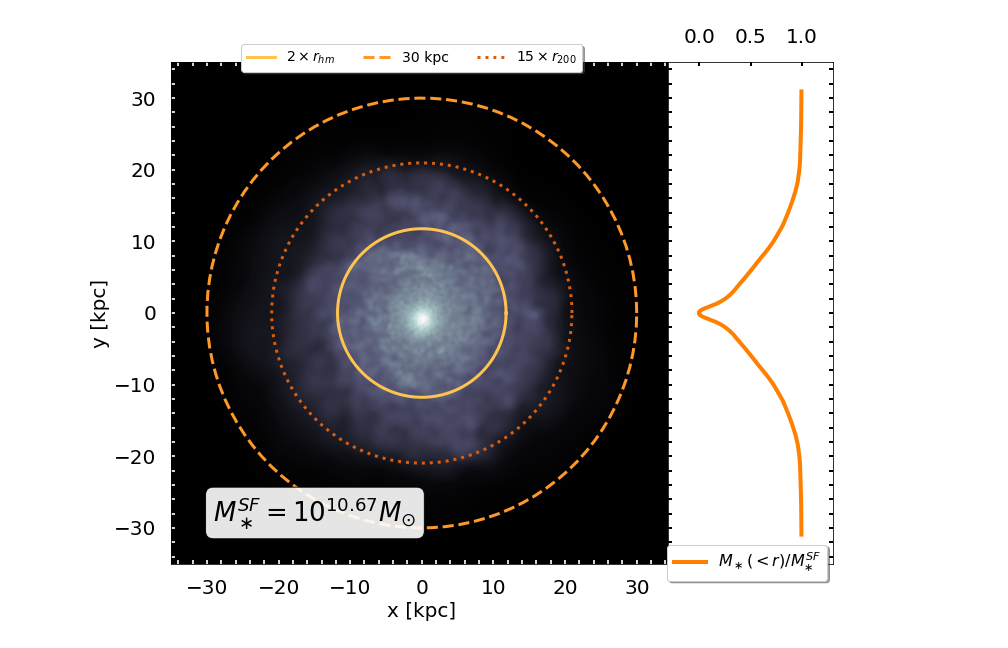
\includegraphics[width=1\textwidth]{images/galaxy_size_disk.png}
    \caption{Left: The stellar mass distribution of a $M_\ast = 10^{10.67} M_\odot$ late type galaxy. The orange lines represent three different galaxy size definitions, $2 \times r^{SUBF}$ (solid line), 30 kpc (dotted line) and $0.15 \times r_{200}$ (dashed line).
    Right: The cumulative stellar mass distribution, divided by the total stellar mass bound to the subhalo, as function of radius.
    }
    \label{gal_size_disk}
\end{figure}

\begin{figure}
    \centering
    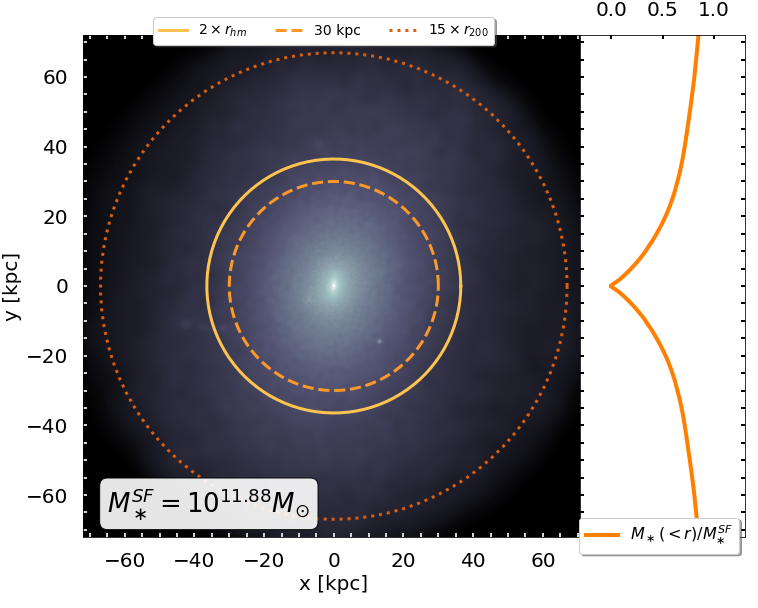
\includegraphics[width=1\textwidth]{images/galaxy_size_big.png}
    \caption{Left: The stellar mass distribution of a $M_\ast = 10^{11.88} M_\odot$ early type galaxy. The orange lines represent three different galaxy size definitions, $2 \times r^{SUBF}$ (solid line), 30 kpc (dotted line) and $0.15 \times r_{200}$ (dashed line).
    Right: The cumulative stellar mass distribution, divided by the total stellar mass bound to the subhalo, as function of radius.
    }
    \label{gal_size_big}
\end{figure}


\subsubsection{Magnitude and colors}

The absolute magnitude ($\mathcal{M}$) is a measure of the total luminosity ($L$) of the galaxy such that $\mathcal{M} = -2.5 \log(L/L_\odot) + \mathcal{M}_\odot$, where $L_\odot$ is the solar luminosity and $\mathcal{M}_\odot$ is the solar magnitude.

For the SUBFIND group catalog, the \texttt{SubhaloStellarPhotometrics} field gives the magnitudes based on the summed up luminosities of all the stellar particles in the subhalo. Eight bands are available, but here only the g- and i-band are used. The g-i colors are then calculated by simply subtracting the i-band magnitude from the g-band magnitude. The color is also computed considering only particles within the $0.15 \times r_{200}$ and 30 kpc aperture.

\subsubsection{Masses}

Stellar mass estimates from observations depend on the stellar initial mass function (IMF), which describe the spectral evolution of a population of stars, and as such the relationship between luminosity and mass in a given spectral band. SAMI and TNG both adopt a \textcite{Chabrier2003} IMF, and so their stellar masses and magnitudes should be comparable without further convertion.

In SUBFIND, masses for each particle type are calculated by summing up all the masses of that particle type belonging to the subhalo. Values for the mass within the stellar half-mass radius, two times the stellar half-mass radius and the radius at which the maximum rotational velocity is found are also available.

Using the particles, the stellar mass within 15 \% of the virial radius ($M_\ast^{15r200}$) and the stellar mass within 30$\,$ kpc ($M_\ast^{30kpc}$) were calculated. These correspond to using a galaxy size limit of 15 \% $r_{200}$ and 30 kpc. These stellar mass definitions, along with the SUBFIND total stellar mass and the SUBFIND stellar mass within two times the SUBFIND stellar half mass radius are all definitions which are commonly used in works where TNG data is employed \parencite[see e.g.,][]{Vazquez2020, Ferrero2020, Lu2020, Rodriguez2020}.

For the SAMI data, the stellar masses are calculated by using the redshift, the i-band magnitude and g-i color of each galaxy through the formula 

\begin{equation}
	\begin{split}
		\log(M_*/M_\odot) = -0.4i + 0.4D - \log(1.0+z) + (1.2117 - 0.5893z) + \\
		 (0.7106 - 0.1467z) \times (g-i), 
	\end{split}
\end{equation}

where $D$ is the distance modulus and $g$ and $i$ are the aperture-matched observed-frame Milky Way-extinction-corrected apparent magnitudes \parencite{Bryant2015}.

\subsubsection{Characteristic size}\label{charsize}

In observational data, galaxy sizes are always projected sizes, as they are derived from 2D images. A common measure of the size of a galaxy is the effective radius ($R_e$), which is the radius within which half the light of the galaxy is contained. This quantity depends on the analysis and quality of the 2D profiles, which may not be able to include all the light in a galaxy in the way that we can ensure for computer simulated data. The radius also depends on which optical filter the measurements are made in, as different filters will be receptive to light from different parts of the galaxy \parencite{Sande2018}. In simulation data, effective radii are more commonly given by the 3D stellar half-mass radius ($r_{hm}$), and so should not be compared directly to observations (which are projected sizes). The stellar half-mass radius is the radius of a spherical volume within which half the stellar mass is found. This value is generally higher than the 2D half-light radius ($R_{hl}$) for a given mass up to $M_{*} < 10^{10.5}$, as seen in \textcite{Genel2017}. A 2D half-mass radius ($R_{hm}$) can be calculated by averaging the projected half-mass radius of the galaxy in three different orthogonal directions. A computationally less expensive method is to just use the approximation $R_{e} = \frac{3}{4} r_{e}$, which generally holds for a range of surface brightness profiles observed in stellar systems \parencite{Wolf2010}. Both 3D half-mass radius and 2D projected half-mass radius were calculated for $M_\ast^{15r200}$ and $M_\ast^{30kpc}$. The SUBFIND catalog provides stellar half-mass radius for $M^{SUBF}_*$.

The SAMI catalog data has two different estimates for effective radius. The first is based on Sérsic fits to SDSS and VST imaging data and is defined as the semi-major axis half-light radius, measured in the r-band. The values are given in units of arcsec which were then converted to a physical radius in kpc. Then these semi-major axis radii are converted to circular radii using the formula

\begin{equation}
   R_{circ} = R_{sm}\sqrt{(1-\epsilon)},
\end{equation}

where $R_{circ}$ is the circular radius, $R_{sm}$ is the semi-major axis effective radius and $\epsilon$ is the eccentricity which is also available for each galaxy.

The other effective radius available in the catalogs is the circularized effective radius calculated from the SDSS and VST photometric data using the Multi Gaussian Expansion (MGE) algorithm, the details of which can be found in \textcite{Scott2021}. These values are on average slightly smaller than the former definition, especially for early-type galaxies.

\subsubsection{Velocities}

Galaxy velocities are usually given by the stellar velocity dispersion ($\sigma_*$) and rotational velocity ($V_{rot}$) for early and late-type galaxies, respectively. This is because of the difference in the shape of the two galaxy types. It makes more sense to talk about velocity dispersion in a spheroidal pressure-dominated system and rotational velocity in a rotating disk.

In the SUBFIND catalog, the field \texttt{SubhaloVMax} gives the maximum value for the spherically averaged rotation curve of a given galaxy. As the rotational curves are nearly flat for large enough radii, it should not be very important at which specific radius the observational rotational velocity is measured, as long as it is in the flat part of the curve. For observational data, the rotational velocities are usually measured in the outer part of the galaxy. A common place to measure is at $2.2\, R_e$ which is the radius of maximum rotation for an isothermal sphere. Using the particles it is possible to study the rotational velocity at any radius, so it was calculated at $2.2\, r_{hm}$ to see if this made a difference in the overall trend compared to \texttt{SubhaloVMax}. 

Rotational velocities were not available in SAMI catalog data, but an extensive analysis of the 2D velocity maps in SAMI DR2 is found in \textcite{Bloom2017}. They defined the rotational velocity as the velocity at $2.2\, R_e$, which should be in the flat regime of the velocity curve, and coincide well with the maximum velocity. Their best fit for the TFR was used in our comparison, 
\begin{equation}
	\log(V_{rot}) = 0.31 \pm 0.0092 \times \log(M_*)-0.93 \pm 0.1.
\end{equation}

The velocity dispersion in the SUBFIND catalog is the 3D velocity dispersion of all the particles over the entire subhalo, divided by $\sqrt{3}$. %why

Assuming that velocity dispersion tends to fall off at larger radii, and the galaxy has an ellipsoid shape, the angle at which the galaxy is viewed will affect the observed velocity dispersion. To compensate for this when comparing simulations to observations, velocity dispersions in simulations may be calculated in three different projections of the galaxy and averaged over these. 

\begin{equation} \label{sigma1}
    \sigma^{2} = \frac{1}{3}(\sigma_x^2 + \sigma_y^2 + \sigma_z^2)
\end{equation}

This was done for the TNG particles, as well as calculating 3D velocity dispersions of each particle type within the entire subhalo, $0.15 \times R_{200}$, $30\,$kpc and $10\,$kpc.

In SAMI catalog data, the given velocity dispersion is averaged within an aperture with radius equal to the effective radius of each galaxy. Both Sèrsic and MGE values are available, but the Sèrsic fits were chosen as a quick comparison to MGE data showed that there was no real difference between the two.

\subsection{Galaxy morphology classifications}

Galaxy morphology is as stated in the previous Section a spectrum, ranging from disks to ellipticals to irregular shapes. It is therefore an impossible task to make an exact division between early and late type galaxies, as such a division does not appear in nature. However, it is still useful to see if the different galaxy types are present in the simulation, and to try to compare their properties to those from observations. In this analysis, a subselection of each galaxy sample (TNG mock galaxies and SAMI observed galaxies) is labeled as ``early type'' and another as ``late type''. The remaining galaxies are ``intermediate type'', and are included in results where all galaxies are analysed. In the case that only early or late types are analysed, this is stated clearly to avoid confusion. The galaxy classification selection process for TNG and SAMI are described in this subsection.

Starting off with the same subset of 7303 TNG subhalos, we get different results for which galaxies are classfied as early- and late-type galaxies, based on the classification method as well as the volume in which the relevant properties are measured. The details are presented in Table \ref{morph}. The selection process using the sSFR with $ -1.44 < \log (sSFR[Gyr^{-1}]) $ being late type and $\log (sSFR[Gyr^{-1}]) < -1.94$ being early type gives very similar results whether the star formation rate and stellar mass is calculated within 30 kpc, $0.15 \times r_{200}$ or the entire subhalo. These findings agree well with \textcite{Schaye2015}, which found the effect of a 30 kpc aperture to be neglible for star formation rates compared to that of the whole subhalo. They do however find stellar mass to be affected, with smaller galaxy apertures giving smaller stellar masses for galaxies with mass $M_* > 10^{11}M_{\odot}$. This would give a slighly larger sSFR to the most massive galaxies when smaller aperture sizes are used, potentially leading to fewer early type galaxies. However, the SFR is already very small in these galaxies so the effect on the selection process is minimal as seen in Table \ref{morph}.

For the classification method using the criteria of late type galaxies having a gas-to-stellar mass fraction $f_{gas} > 0.1$ and early types having $f_{gas} < 0.1$ to separate the galaxies we get a much more profound difference by using different apertures when calculating $f_{gas}$. Especially for the values which are available using SUBFIND catalog values only, there is a huge difference in the selection. This is because there is a large difference in where the gas and stellar particles are situated within the halo, with the majority of the gas mass being found in the outer part of the galaxy where there are few stars.

By using the simple cut at $\kappa_{rot} = 0.6$ we get a completely different result from the two methods above, where there was a majority of late-type galaxies. In real life we know that smaller late-type galaxies dominate, so using only the rotational energy does not yield the expected ratio. However, combining this result with one of the two above should result in a subset of galaxies which exhibit both the right amount of cold gas and the star formation that goes with it, as well as the expected kinematic structure.

In the rest of this paper, TNG early-type galaxies are those which, calculated using the particles and an aperture of 30 kpc, have a sSFR of $\log (sSFR[Gyr^{-1}]) < -1.94$ as well as $\kappa_{rot} < 0.6$. TNG late-types have a sSFR of $ -1.44 < \log (sSFR[Gyr^{-1}]) $ as well as $\kappa_{rot} > 0.6$. This results in 1336 early-type galaxies, 1449 late-types and 4518 intermediate-type galaxies.

%consider including an extra pair of columns called (sSFR+K_rot) highlighting these numbers used in the rest of the paper. It is not too straightforward to compared f_Gas and k_rot with sSFR because the former classification way also flag "intermediate type" while the others not.
\begin{table}
\begin{center}
\caption{The number of early (E) and late (S) type galaxies in the sample of 7303 galaxies for different classification methods and volumes within the classifying properties are calculated within. Values marked with * are available through the SUBFIND catalog.}
 \label{morph}
\begin{tabular}{ l| c c c c c c c c c } 
 \hline
 \hline
   &\multicolumn{2}{c}{sSFR}&\multicolumn{2}{c}{$f_{gas} = 0.1$}&\multicolumn{2}{c}{$\kappa_{rot} = 0.7$}&\multicolumn{3}{c}{$sSFR+\kappa_{rot}$}\\
   &  E & S & E & S & E & S & E & S &I  \\
 \hline
 $r_{hm}^{SUBF}$ & - & - & 2493* & 4811* & - & - & & & \\ 
 2 $\times r_{hm}^{SUBF}$ & - & - & 1847* & 5456* & - & - & & & \\ 
 30 kpc & 1493 & 5213 & 864 & 6439 & 5554 & 1749 &1335 & 1453 & 4515 \\ 
 15\% r$_{200}$ & 1497 & 5212 & 817 & 6486 & 5582 & 1721 & 1342 & 1426 & 4535 \\ 
 Subhalo & 1491* & 5201* & 80* & 7224* & - & - & & &\\ 
 \hline 
 \end{tabular}
\end{center}
\end{table}

SAMI DR3 provides its users with a catalog of visual morphology classifications which members of their team have performed. It is relatively simple with four galaxy types; ellipticals, S0s, early spirals and late spirals, as well as an ``unknown'' category. This last category comprises only about 5\% of the sample. In this work, the galaxys are further separated into just two categories, early and late type galaxies, where the former contains ellipticals and S0s while the latter contains only late spirals. This gives a total of 1216 early types, 435 late types and 1415 intermediate types.